\documentclass{article}

\usepackage{mathtools,amsfonts}
\usepackage{enumerate}
\usepackage{fancyvrb}
\usepackage{graphicx}
% \usepackage{fullpage}
\graphicspath{ {./} }


\begin{document}
\thispagestyle{empty}

\begin{center}
  \textbf{\Large Junior Test 2}
  % LEVEL is Senior, Intermediate or Beginner
  % NUMBER is the test number: 1, 2, etc.
  \\ \vspace{1em}
  \textbf{\large Stellenbosch Camp 2019}
  \\ \vspace{1em}
  \textbf{\large Time: $4$ hours}
\end{center}

\vspace{6.81mm}

\begin{enumerate}[1.]

\item %
Tile an $8 \times 8$ chessboard with T-shaped tetrominoes, which look as follows:
\begin{center}
	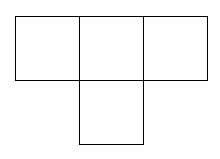
\includegraphics[scale=0.3]{test_2_q_1.png}
\end{center}


\vspace{6.81mm}

\item % 
Prove that for all $a, b > 0$
\begin{center}
$\frac{a}{b} + \frac{b}{a} \geq 2.$ 
\end{center}
\vspace{6.81mm}


\item % 
In $\triangle ABC$ let $\angle ACB = 90^\circ$, $AC = 1$ and $AB = 2$.

Let $M$ be the midpoint of $AB$ and $D$ the intersection of the angle bisector of $\angle CAB$ and $BC$.

Prove that $AB \perp CM$.


\vspace{6.81mm}


\item % 
Find the first number which appears in all 3 the following arithmetic progressions:
\begin{center}
	$21, 34, 57, 70,...$\\
	$33, 37, 41, 45,...$\\
	$42, 75, 108, 141,...$
\end{center}
\vspace{6.81mm}

\item %
There are 7 people A, B, C, D, E, F, and G sitting in a row. B wants to sit next to C and E wants to sit next to F. How many different seating arrangements are there?
\vspace{6.81mm}

\item %
Given $\triangle ABC$, with $AB < AC$, let D be the point where the angle bisector of $angle BAC$ intersects the circumcircle of $\triangle ABC$.
Let $P$ and $Q$ be the altitudes dropped onto the extensions of $AB$ and $AC$.
Prove that $PB = QC$.

\vspace{6.81mm}

\item %
What are the last two digits of $7^{7^{7^{7}}}$?
\vspace{6.81mm}

\item %
Prove that for all $a, b, c, d > 0$,
\begin{center}
	$(a + b + c + d)^{4} \geq abcd \times 4^{4}$
\end{center}

\item % Emile, C
Given the below colouring, is it possible to invert the colours of rows or the colours of columns in some order to achieve a completely white board?
\begin{center}
	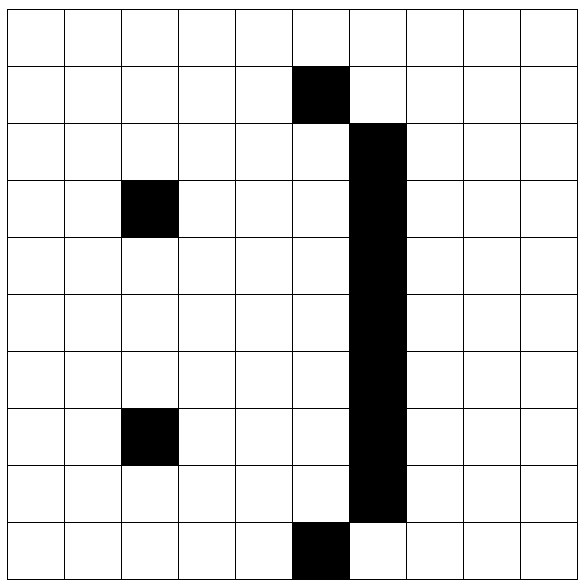
\includegraphics[width=0.5\textwidth]{test_5_q_1.png}
\end{center}

\vspace{6.81mm}

\item % , 2018 December Monthly Assignment Q1
Let $n$ be a positive integer greater than 2. Let $r_1$ be the smallest odd divisor of $n$ greater than $1$ and let $r_2$ be the largest odd divisor of $n$. Find all $n$ such that
\begin{center}
	$n=5r_{1}+3r_{2}$.
\end{center}


\end{enumerate}


\vfill
% ASCII art
\begin{center}
\begin{BVerbatim}
   .___,   
___('v')___
`"-\._./-"'
    ^ ^ 

\end{BVerbatim}
\end{center}

\end{document}
